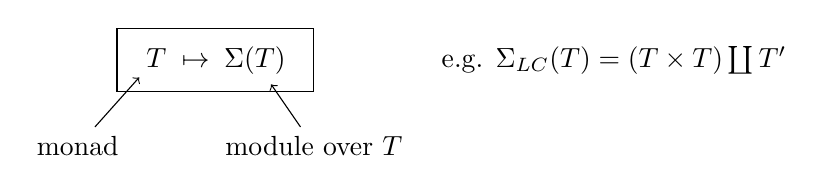
\begin{tikzpicture}[->]
% \node (v2) at (0,0) {$\boxed{T\mapsto \Sigma(T)}$};
\node (v1) at (-0.5,-1) {monad};
\node (v2) at (2.5,-1) {module over $T$};
\node[anchor=base] at (1,0) {$\mapsto$};
\node[anchor=base] (v3) at (1.75,0) {$\Sigma(T)$};
\node[anchor=base] (v4) at (0.5,0) {$T$};
\draw  (v2) edge (v3);
\draw  (v1) edge (v4);
\draw  (0,0.5) rectangle (2.5,-0.3);
\node[anchor=base west] at (4,0) {e.g. $\boxed{\Sigma_{LC}(T)=(T\times T)\coprod T'}$};
\end{tikzpicture}